\documentclass{article}

% Language setting
% Replace `english' with e.g. `spanish' to change the document language
\usepackage[english]{babel}

% Set page size and margins
% Replace `letterpaper' with `a4paper' for UK/EU standard size
\usepackage[letterpaper,top=2cm,bottom=2cm,left=3cm,right=3cm,marginparwidth=1.75cm]{geometry}

% Useful packages
\usepackage{amsmath}
\usepackage{graphicx}
\usepackage[colorlinks=true, allcolors=blue]{hyperref}
\usepackage{xcolor}

\title{\textbf{SEMINAR REPORT TITLE}\\
Seminar Report}

\author{TEAM:\\
1st student name, first1.last1@ubbcluj.ro\\
2nd student name, first2.last2@ubbcluj.ro\\
3rd student name, first3.last3@ubbcluj.ro\\
4th student name, first4.last4@ubbcluj.ro
}



\newpage

\begin{document}
\maketitle

\textcolor{red}{\textbf{Important notes:}
\begin{enumerate}
    \item For a team of 4 students the seminar report should have 10+ pages, meaning min. 2.5 pages for each contributor, without counting the first page (Title \& Contents section) and the last page (References section).
    \item Please include in the \textbf{Conclusions} section the summary of the contributions of each student.
    \item \textit{While elaborating the seminar report} - please engage in the tasks such that the final version of the report consists of details presented in clear manner. Assuming that you were the reader of the report (1) you should be able to understand the content and (2) you should be able to apply easily (if needed).
    \item Please provide a meaningful title for the seminar report, i.e., SEMINAR REPORT TITLE.
    \item \textit{When turning in the report} - no slides for the presentation of the report are required. You may navigate over the file and present it. You may organize the presentation the way you want, e.g., one student presents the entire report or several team members discuss different sections of the report. The entire team must attend the seminar report presentation.
    \item Please remove from the final version of the seminar report all instructions written in \textcolor{blue}{blue} or \textcolor{red}{red}.
\end{enumerate}
}

\tableofcontents

\newpage

\section{Introduction}
\label{label:Introduction}

\textcolor{blue}{Include a paragraph with details about the topic approached. Discuss in another 1-2 paragraphs the relevance of the topic within the security domain.
}


\section{Related Concepts / Previous Work}
\label{label:RelatedConcepts}

\textcolor{blue}{\textit{For the practical approach} $->$ Introduce the most important concepts related to the addressed topic. Include references where required and cite them in this way \cite{greenwade93}.\\
\textit{For the research approach} $->$ Provide a short summary about previous research results. Use 2+ papers and cite them \cite{Vuln001}.
}


\section{\textit{Topic-based Sections}}
\label{label:TopicBasedSection}

\textcolor{blue}{\textit{For the practical approach} $->$ Include \textit{in extenso} details about the targeted topic. If needed, use additional sections and subsections.\\
}

\textcolor{blue}{\textit{For the research approach} $->$
Describe the contributions, compare approaches of the papers reviewed.
}

\subsection{Examples / Results}

\textcolor{blue}{Where needed, please include examples and experiment results using tables (Table \ref{tab:TCs1}) and screenshots or images (Figure \ref {fig:frog}) and cite them. }

\begin{table} [htpb]
\centering
\begin{tabular}{l|l|l|l|l}
Feature & TC ID & Input1 & Input2 & Expected Output \\ \hline
F001  &TC01 & 42 & 15 & 100\\
F001  &TC02 & 1 & -2 & 3\\
F002  &TC03 & 111 & 90 & -74
\end{tabular}
\caption{\label{tab:TCs1}TCs table.}
\end{table}

\begin{figure} [htpb]
\centering
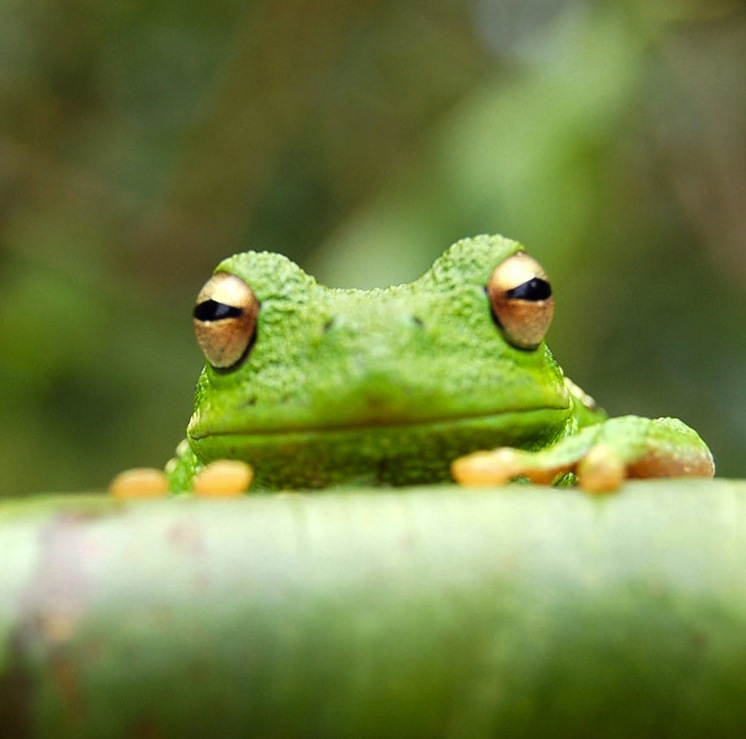
\includegraphics[width=0.25\linewidth]{Figures/frog.jpg}
\caption{\label{fig:frog}This frog was uploaded via the file-tree menu.}
\end{figure}


\section{Conclusions}
\label{label:Conclusions}

\textcolor{blue}{Include conclusions about the investigated topic, lessons learned, and personal considerations while working as a team on the selected topic, summarized in 3-4 paragraphs. When listing the contributions of each team member, you may have something like this:}

\textcolor{blue}{\begin{itemize}
\vspace{-0.5cm}
    \item 1st student name - sections \ref{label:Introduction} and \ref{label:RelatedConcepts}
    \item 2nd student name - sections \ref{label:RelatedConcepts}, \ref{label:TopicBasedSection}, and \ref{label:Conclusions}
    \item etc.
\end{itemize}}

\section{Other sections...}

\textcolor{blue}{Please remove this section and all subsections.}
\subsection{How to include Figures}

First you have to upload the image file from your computer using the upload link in the file-tree menu. Then use the includegraphics command to include it in your document. Use the figure environment and the caption command to add a number and a caption to your figure. See the code for Figure \ref{fig:frog} in this section for an example.

Note that your figure will automatically be placed in the most appropriate place for it, given the surrounding text and taking into account other figures or tables that may be close by. You can find out more about adding images to your documents in this help article on \href{https://www.overleaf.com/learn/how-to/Including_images_on_Overleaf}{including images on Overleaf}.


\subsection{How to add Citations and a References List}

You can simply upload a \verb|.bib| file containing your BibTeX entries, created with a tool such as JabRef. You can then cite entries from it, like this: \cite{greenwade93}. Just remember to specify a bibliography style, as well as the filename of the \verb|.bib|. You can find a \href{https://www.overleaf.com/help/97-how-to-include-a-bibliography-using-bibtex}{video tutorial here} to learn more about BibTeX.

If you have an \href{https://www.overleaf.com/user/subscription/plans}{upgraded account}, you can also import your Mendeley or Zotero library directly as a \verb|.bib| file, via the upload menu in the file-tree.

\newpage

\bibliographystyle{alpha}
\bibliography{sample}

\end{document}